\chapter{literaturereview}
\section{Abstract}
The purpose of this literature review is to analyse information gathered across five
different papers related to Java compatible frameworks. The papers titled,
\begin{itemize}
	\item “Patterns of cross-language linking in java frameworks”\cite{patterns} 
	\item “A Presentation Framework to Simplify the Development of Java EE Application Thin Clients”\cite{thin}
	\item “Developing Java EE Applications Based on Utilizing Design Patterns”\cite{designpatterns}
	\item “J2EE development frameworks”\cite{j2ee}
	\item “Spring framework for rapid open source J2EE Web application development: a case study”\cite{spring}
	\end{itemize}
	
	Will help illuminate and further develop my understanding of JEE applications, JEE compatible frameworks, design patterns in Java and indepth knowledge regarding specific frameworks.
	
	I will start by reviewing the paper with the least relevance and connect the points most closely related to my project. Linking features of each paper to display an understanding of what has been covered and what is undocumented in the field my project resides.
	
	\section{Introduction}
	
	\subsection{General Topic}
	Java EE applications are large and often difficult to understand due to their complexity. Employing Java compatible frameworks in the development of an application can reduce the complexity and assist in creating a more efficient, cost effective application.
	It’s not enough to just begin developing an application with any compatible framework. Frameworks come in many different shapes, sizes, tools, components. Many factors must be considered in selecting the correct framework to incorporate in to the application development. 
	
	\subsection{Introduction to Literature}
	“Patterns of cross-language linking in java frameworks” argues that little research has been carried out on the development of cross language links. During the development and maintenance of applications using a framework to connect multiple languages it is imperative to keep links intact. The inability to understand the connections in the framework where different languages meet affects productivity, efficiency and future development. The paper identifies common patterns in cross language linking in the domain of Java frameworks. Although the aim is to further explain cross language linking, the authors develop through their main research question exclusively in Java.
	
	“A Presentation Framework to Simplify the Development of Java EE Application Thin Clients” has the aim of ultimately creating a framework to develop JEE applications that support the presentation tier. In doing so the authors carry out an extensive survey on all existing presentation tier frameworks compatible with Java. In order to create the framework, they examine and compare features of Struts and Spring frameworks. Further this paper examines Java Server Faces (JSF) and JEE Design Patterns.
	
	“Developing Java EE Applications Based on Utilizing Design Patterns” concerns the selecting and implementing of design patterns in Java EE applications. The paper describes the Model View Controller (MVC) with integration from Spring and Hibernate. Analyzing multiple design patterns and validate the feasibility of the framework model for implementation.
	
	“J2EE development frameworks” was published in 2005 and discusses the topic of J2EE providing a lack of programming support for developers. This paper explains many of the factors that led to open source framework being created and implemented. Topics in this paper cover the emergence of open source frameworks, the reason why open source frameworks are needed and 3 popular open source Java compatible frameworks (namely Struts, Hibernate and Spring). Further the paper discusses what is next for open source frameworks and standard J2EE frameworks.
	
	“Spring framework for rapid open source J2EE Web application development: a case study” compares the features of Spring and J2EE Enterprise Java Beans (EJB). The authors examine the EJB architecture necessary to run an EJB and lightweight container architecture which can run the Spring framework. Describing the goal of the Spring framework as developing an application as accurately, efficiently and as economically as possible.
	
	\subsection{Reason for Literature Review}
	I am currently a 4th year student compiling a thesis on Java compatible frameworks. In my project I am comparing four Java frameworks, cross referencing features, components, usability, community support and application development. After comparing the four frameworks I will implement one of the frameworks in to a prototype application to showcase the features of the chosen framework. 
	
	I hope that reviewing these five papers will further my understanding of the core principles of integrating a JEE compatible framework in to my prototype application. From the papers I have chosen there are clear connections between how to compare frameworks, why frameworks came to exist, how frameworks should be implemented and good design principles that coexist with framework development.
	
	\newpage
	
	
	\section{Literature Review}
	
	\subsection{Patterns of Cross Language Linking in Java Frameworks}
	
	\subsubsection{Introduction to Cross Language Support}
	To understand Mayer and Schroeder’s motivation for undertaking this project we must understand that very little has been written in the area of cross language support. This lack of support is detrimental to the developers and the systems stability \cite{crosslanguagecodeanalysis}\cite{tamingofconfusion}. Although Mayer and Schroeder set out to understand how links between artifacts (in this case class, subclasses and components) are formed among different programming languages. They also ask the question if links share characteristics and can be similarly described.
	
	\subsubsection{Choosing Frameworks}
	Instead of choosing two different programming languages fearing that the scale of the project may be too large. The project incorporates frameworks all written in one language but incorporating unique classes. For the chosen frameworks the authors used theoretical sampling. This allowed the inclusion of three well defined and well used industry frameworks, Android UI, Spring and Hibernate. This seemed a logical choice due to the good documentation, support and open source resources of all three frameworks.
	
	\subsubsection{Defining and Testing}
	Defining what a link is was an important step. Having tangible characteristics for a link allowed Mayer and Schroeder to draw UML diagrams displaying how links interacted, where they interacted and what was expected to happen. Without coding anything it could be possible to understand what a line of java code from a framework interacting with an artifact in the standard library might look like.
	
	Three applications were implemented with each framework. The applications were connected to each framework respectively {(OpenMettings, Spring), (JTrac, Hibernate), (Wordpress, Android)}. Connectivity was checked to ensure that language adapters could be connected to the application to view the entire UML to ensure discovery any unforeseen links. Figure 3.1.1 shows the three frameworks and existing lines of code.
	
	\begin{figure}[!htb]
		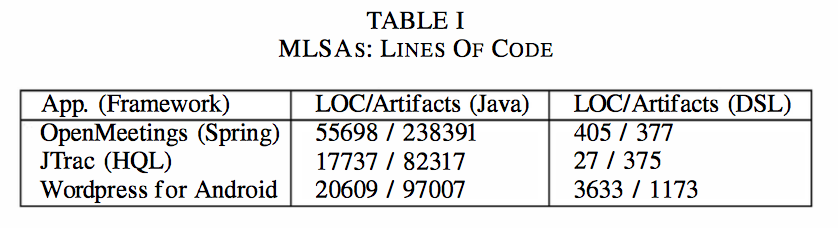
\includegraphics[width=.8\textwidth]{img1.png}
		\begin{center}
			\figurename{ 3.1.1}
			\end{center}
			\end{figure}
			
			Understanding of how a Java object might call another Java object is key to the understanding of this project. Three patters were defined to determine link categories. Eight sub patterns define the link characteristics further. Well structured definitions accommodated good documentation and clear link interactions. 
			
			An example of a Structural link would be if an Object in a Class belonging to OpenMeetings called an artifact of the Spring framework class it would use the defined “For and Find” pattern under Structural. What happens in this interaction is the Object may call a Class in Spring (For) which can call an Object (Find) but that object may have a default constructor so another (Find) is needed with the correct parameters. Figure 3.1.2 shows the structural pattern break down.
			
			\begin{figure}[!htb]
				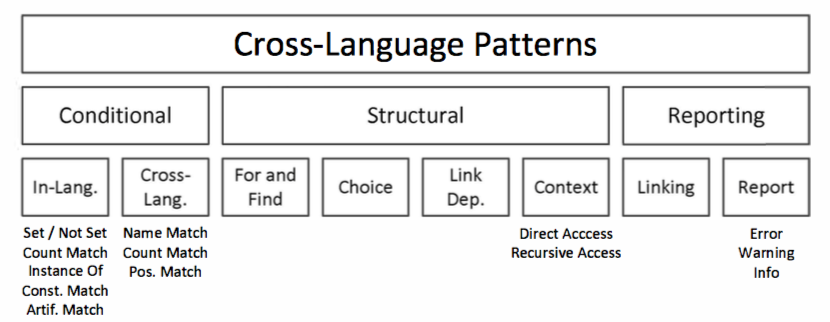
\includegraphics[width=.8\textwidth]{img2.png}
				\begin{center}
					\figurename{ 3.1.2}
					\end{center}
					\end{figure}
					
					\subsubsection{Research Paper Conclusion}
					The paper showed a clear understanding for what was required to identify the characteristics of cross language links between Java and domain specific languages in frameworks. Further the second research question was also able to be answered by categorizing the links regarding their properties. 
					
					\subsection{A Presentation Framework to Simplify the Development of Java EE Application Thin Clients}
					
					\subsubsection{Introduction to MVC Model}
					This paper details the building of a software framework to simplify development at the presentation layer of a Java EE application thin client. The paper begins by explaining design principles of presentation layer in applications namely the Model View Controller (MVC). The MVC is a design model used with graphical user applications to separate data access from business logic displayed to users. The authors agree that the MVC model brings a lot of advantages for application design but concede that the flaws within the MVC are the reason they wish to develop a framework to overcome deficiencies in the MVC design.
					
					\subsubsection{Researched Frameworks}
					To begin developing the framework the paper describes existing Java compatible frameworks designed to simplify development at the presentation layer. As a starting point they survey and analyze these frameworks. The first framework reviewed is Struts 2 \cite{struts}. Struts architecture can be seenin Figure 3.2.1 
					
					\begin{figure}[!htb]
						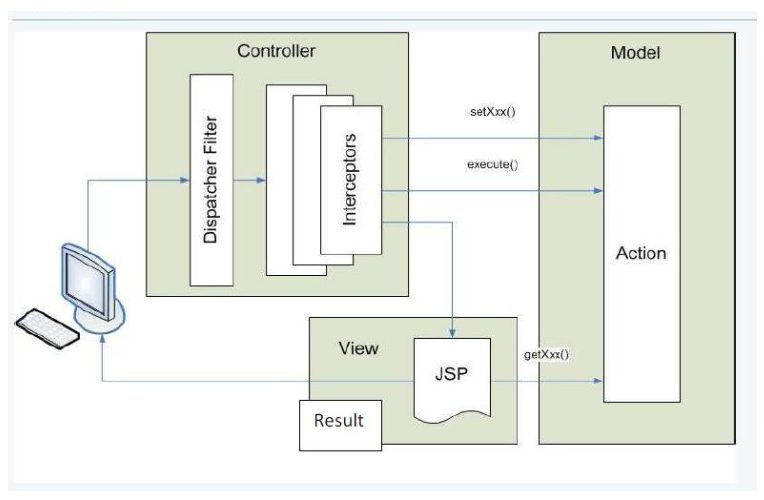
\includegraphics[width=.8\textwidth]{img3.png}
						\begin{center}
							\figurename{ 3.2.1}
							\end{center}
							\end{figure}
							
							Apache Struts 2 is a framework intended to aid in the development of web applications. The paper suggests that Struts automates and reduces tedious development work. Struts also provides an architectural workflow within JEE applications making them more robust and flexible. The paper continues examining the features of Struts with further details regarding Struts ability to work with other frameworks, how actions are used as a core feature to provide functionality back to the user on the view end and finally discuss how Struts use tag libraries to validate inputs for return of dynamic data. 
							
							The next framework reviewed is Spring \cite{springwalls}. Spring uses simple JavaBeans instead of Enterprise JavaBeans. Reducing the number of complex methods as all objects in Spring are considered Plain Old Java Object (POJO) equal to a simple Java class. The authors provide the four strategies that spring proposes to reduce complexity. Use of templates, declarative code, weak coupling by injecting dependencies and light weight development with POJO’s. Springs core architecture can be seen in Figure 3.2.2
							
							\begin{figure}[!htb]
								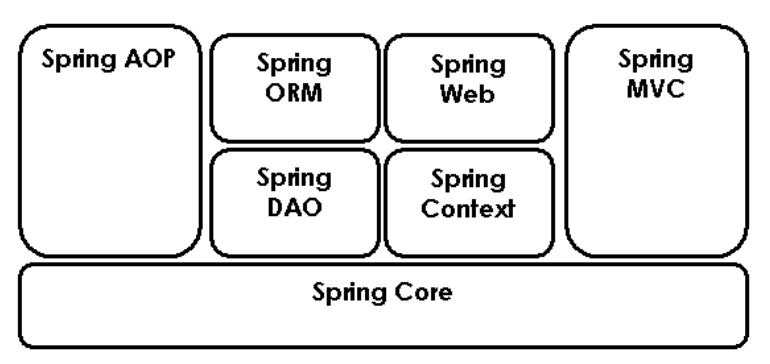
\includegraphics[width=.8\textwidth]{img4.png}
								\begin{center}
									\figurename{ 3.2.2}
									\end{center}
									\end{figure}
									
									Before moving on to design patterns the final framework the authors examine is Java Server Faces (JSF). JSF’s are the Java standard class that was incorporated into Java EE 5. The purpose of JSF’s is to allow development of Java web applications in a similar fashion to desktop applications. Webpage updates are managed by the framework which translates user actions in to messages sent from the server. Advantages with JSF include being the Java EE standard, having a set of UI tools and allow integration of third party components.
									
									These frameworks provide features that the authors wish to implement in to the framework they are developing. Some features of certain frameworks lend themselves closer to developing at the presentation layer of JEE applications but no framework is a perfect match. Design patterns exist to provide solutions to problems with a given level of functionality\cite{designpatternshall}. In order to correctly complete the framework, the paper next describes the design patterns to be implemented along with the chosen framework. 
									
									\subsubsection{Creating the JEE Application}
									The ability to define the requirements needed for the framework greatly improves the accuracy of the deliverable. The authors declare a list of features they wish to incorporate in to their framework. During the description of the existing frameworks, each examined framework had a bullet point list of advantages and disadvantages. So comparing the features they wish to develop in to their own framework against the features in the existing frameworks can help narrow the path of the project. This was a good step for project development. Clearly defining features to cross reference.
									
									After listing the requirements for their framework it was concluded that the existing framework they would follow closest was Struts. In order to develop their framework further to accommodate the simplification of development at application layer the paper next describes incorporating the design models in to the framework design.
									
									The framework developed used features of struts in forms and actions. With each action defining the result much like the JSF. Along with the code from existing frameworks, following design patterns allowed this framework to simplify development at presentation layer. The authors declare that their framework achieves better results than simply using Struts. They pair their hybrid framework with the service to worker design model, allowing easy parameterized navigation through results, attributes, invocation and validation.
									
									\subsubsection{Research Paper Conclusion}
									I feel this paper gives good detail behind the processes need when developing an application. The authors correctly identified a design pattern to develop their application around. Researching and explaining the frameworks they chose and why they were chosen to benefit the development was well documented. Additional information was provided with patterns they chose not to use. The information was helpful in explaining why they didn’t choose the intercepting filter or JSF.
									
									The paper explains future work being related to developing larger full web applications in various domains to gain feedback within multiple areas of the framework. This shows that external of the allocated project time the authors had developed the idea of a complete application.		
									
									\subsection{Developing Java EE Applications Based on Utilizing Design Patterns}
									
									\subsubsection{Introduction to Application}
									This paper is based on a theoretical project to build a pilot management application in JEE. The application manages ship captains and drivers at a busy port in China. Storing data on captains working and available. Development of the application will be done through Spring and Hibernate frameworks along with several design patterns to be adapted in to the application.
									
									\subsubsection{Introduction to Design Patterns}
									The paper begins with discussion of design patterns explaining how important patterns fit in to the software development process and how design patterns are leveraged to solve system design problems. When selecting a design pattern the first consideration should be how does the design pattern solve the design problem. The authors suggest that after assessing multiple possible solutions, the option of a hybrid variable mixing components of multiple design patterns together should be considered.
									
									\subsubsection{JEE and Framework Selection}
									The project uses frameworks which the authors claim lends its self to greater abstraction and therefore further reuse. Using the MVC\cite{MVC} pattern and Spring, an open source framework comprised of a layered architecture. This feature allows spring developers to be selective over which components are used and yet still maintains a robust framework for JEE applications. For storage the project uses Hibernate framework as a relational mapping tool for Java. Hibernate accommodates standard Java expressions with abstraction, inheritance, polymorphism, and the Java collections framework. Hibernate greatly reduces development time relating to persistence data storage. Hibernate provides commands to store and retrieve data along with the mapping of classes to database tables.
									
									The authors discuss the importance of EJB in JEE application design but with the rise of open source frameworks along come the abilities to create superior applications with less cost. Declaring the open source frameworks provide more tools, are more simple to learn, more simple to use and are in the end more flexible. The authors claim that Spring and Hibernate are the appropriate tools for developing this application.
									
									\subsubsection{Design Pattern Selection}
									When selecting their design pattern the authors suggest following a 7 step rule.
									\begin{itemize}
										\item Study the pattern
										\item Study the structure, participants  and collaborations 
										\item Look at concrete example of the pattern
										\item Choose names that are meaningful to application for classes
										\item Define the classes
										\item Define application specific names for methods in operations in the pattern
										\item implement the operations to carry out the responsibilities and collaborations in the pattern
										\end{itemize}
										
										\subsubsection{Research Paper Conclusion}
										The paper gives good basis for designing application with frameworks. The paper tends not to go in to specifics of the frameworks chosen to develop applications but does explain how design patterns should be assessed when designing an application. Seven steps when choosing a design pattern are provided. Explaining their specific platform is well documented with code snippets and generic information about connecting the frameworks to the application. The paper does not explain any future implementation of the application for further development.
										
										\subsection{J2EE development frameworks}
										
										\subsubsection{Introduction to JEE and JEE compatible Frameworks}
										In this paper the author discusses JEE compatible frameworks and reasons they have become so popular. Covering three well used frameworks in the Java developer’s community the author discusses their features, their formative stages and their place in Java application development. Building on top of Java Standard Edition (JSE), JEE fails to import features that allow JSE to work so well with relational databases. Which led to Sun Microsystems promoting Entity Java Beans (EJB) as a standard to aid in the development of applications working with Java Transaction API, Java Naming, Directory Interface etc. Unfortunately, EJB’s remain cumbersome and complex in implementation. EJB’s put constraints on inheritance and complications in unit testing. 
										
										The inability to provide a standard framework that meets all needs of Java application development has proved the impetus for creating open source frameworks that focus on tiers, and individual components of application development. It can be complex to develop a framework for building entire applications and have the end developers experience remain unaffected. Many smaller vendors opt against standard development tools and choose open source solutions that reduce cost and complexity during development. A framework is made of classes that allow applications to have utilize reusable design (normally for one tier).
										
										\subsubsection{Why Use Frameworks}
										The paper provides advantages of using frameworks in application development. The ability for developers to focus exclusively on code specific to their application and not infrastructure. Frameworks can provide structure to code and clear for future development. Easy to follow can promote best practice through community support and documentation. With these advantages along with popular frameworks like Hibernate, Spring and Struts having an important role in JEE development, developers have recognized an area that can reduce cost, provide support, reduce licensing fees all on open source frameworks that are better tested than in house code.
										
										Going in to detail on the frameworks mentioned above, the author provides context and history for the frameworks. Beginning with Struts a web application framework developed in 2000. Deficiencies were evident in the standard Java Server Faces (JSF) model. The connection between business logic and HTML restricted features. Creating a web MVC to move business logic to its on class and separate the HTML. Struts solved this issue well enough to become the popular choice when developing web applications. 
										
										Hibernate is the next framework examined. Java Database Connectivity (JDBC) is the standard provided by Java for communication with databases. The JDBC forces developers to use relational concepts in code, this restricts object oriented design. Further, JDBC is complex and prone to errors when used directly e.g. resource management and exception handling. Hibernate provided a fully featured Object Relational Mapping (ORM) solution to persistence storage. Hibernate provided an intuitive model if not the most innovative. Building on an already existing ORM model but reinforcing and making a more robust framework for persistence solutions within application development.
										
										With Struts and Hibernate in place a Java web application now just needed support for business logic. Java provides a EJB’s but as the paper discussed earlier, EJB’s introduce restrictions and complications during testing. An open source framework exists namely Spring. Spring allows Plain Old Java Objects (POJO) along with Inversion of Control (IoC) and Aspect Oriented Programming (AOP) to decouple the classes from JEE environments. Allowing the POJO to be reused in many different environments. Spring is considered a lightweight container, combining IoC and services. Lightweight containers lend themselves to a much simpler unit testing experience and have been a major factor in the frameworks popularity.
										
										\subsubsection{Reseach Paper Conclusion}
										This paper provides information on how frameworks devloped out of neccesity. Three prominent frameworks in JEE application development are described in detail. Although the paper does not implementation of frameworks it is well documented what the frameworks features are and when they are used in applications. The paper doesn't provide any references but has been cited in many external papers. Concluding with what is next for frameworks gives an insightful view in to how frameworks are constantly evolving through open source rather than specifications. The author explains how framework features such as Aspect Oriented Programming (AOP) are becoming more important.
										
										\subsection{Spring framework for rapid open source J2EE Web application development: a case study}
										
										\subsubsection{Introduction to JEE Frameworks}
										In this paper the authors argue that creating JEE applications as economically, efficiently and as accurately as possible often depends on implementing a framework during development. The implementation of a framework can increase productivity and decrease complexity\cite{experteoneonone}. The paper focuses on Spring, the foremost alternative to creating a JEE compatible web application with out using Enterprise Java Beans (EJB). The paper described the architecture behind Spring and presents a Spring case study.
										
										In order for an application to be considered JEE compliant, three core features of a JEE application must be featured namely the presentation layer, the business layer and the data storage layer. Before introducing the Spring architecture the authors present the descriptions for the EJB architecture and the lightweight container architecture to help familiarise the differences between both developments. Regarding the EJB architecture more detail concerning the three core features components are given. The presentation layer contains the User Interface (UI) tier, the business services contains the business logic methods to allow the UI to interface with the data access layer containing the Enterprise Information System (EIS). A lightweight container invokes an Aspect Oriented Programming (AOP) interceptor to provide services. Doing so enables the ability to add additional behaviour either side of the business methods execution. AOP interceptors are usable outside of any container therefore have no need to use the containers API. Figure 3.5.1 shows EJB architecture with all 3 core components. While Figure 3.5.2 shows EJB lightweight container with MVC framework
										
										\begin{figure}[!htb]
											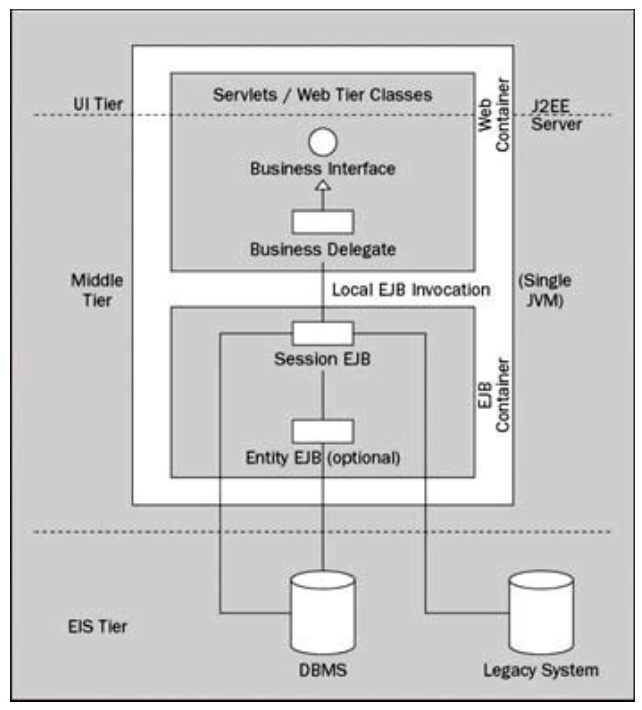
\includegraphics[width=.8\textwidth]{img5.png}
											\begin{center}
												\figurename{ 3.5.1}
												\end{center}
												\end{figure}
												
												\begin{figure}[!htb]
													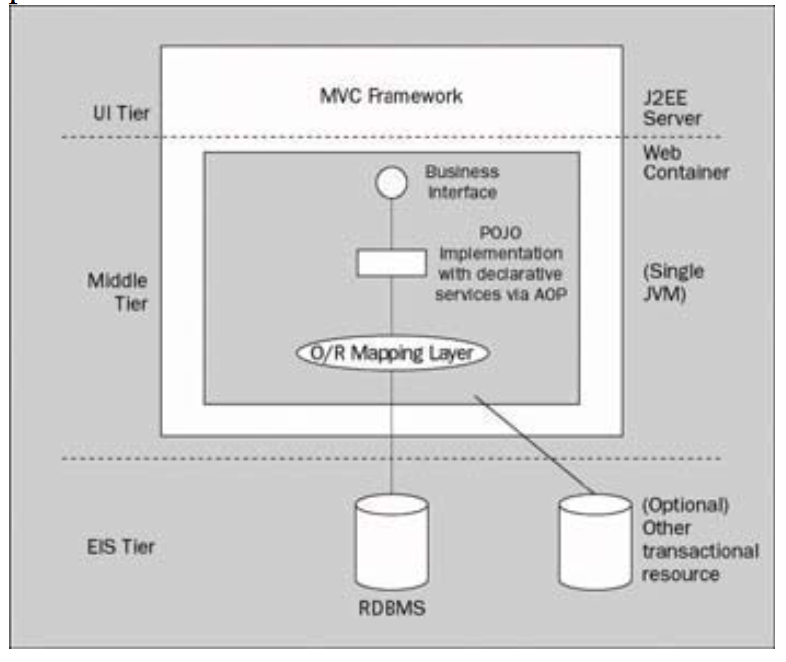
\includegraphics[width=.8\textwidth]{img6.png}
													\begin{center}
														\figurename{ 3.5.2}
														\end{center}
														\end{figure}		
														
														Comparing the differences between standard EJB development and development with a framework comes down to three important objectives, simplicity, testability and portability. EBJ’s are complex and require an EJB container meaning they need a high spec server that can handle additional resources. Lightweight frameworks only require a servlet engine reducing administrative complexity and addresses the issue of portability. When testing business logic EJB’s become obstructed by the fact implanting classes are dependant on an EJB container. With lightweight framework being written as Plain Old Java Objects (POJO)’s it means testing can be carried out external of the application server.
														
														\subsubsection{Spring Framework}
														The authors argue the case that Spring architecture provides a more intuitive developer experience citing claims form one of the authors that, he tried to develop an EJB application in the past and found the experience confusing and obtuse. Later the author developed an application implementing Spring and found he was able to produce more complex code faster and more easily.
														
														Being able to develop code faster and with more ease is dependant on a key feature of Springs framework; Inversion of Control (IoC). The authors describe IoC with a Hollywood principle: “Don’t call us, we’ll call you”. In JEE development there are two types of Ioc, dependency lookups and dependency injections.
														
														First the authors define what differentiates the dependency lookup from the dependency injection. Dependency lookups use container dependant APIs to look up resources. The container provides component call-backs and a lookup context. Managed objects must do their own lookups. This form of IoC differs from dependency injection where the objects are not responsible for looking up their resource or other dependencies.
														
														The application code is separated from the resource lookups. This allows the objects to be used outside of the container with no need for APIs. Furhter information regarding types of IoC depedancy injection are defined; Setter injection and constructor injection. Setter injections are invoked once the object is instantiated by the container. Constructor injection needs arguments passed through the constructor to define the dependencies.
														
														\subsubsection{Case Study Development}
														Developing the case study in Spring allowed the authors to showcase the setter injection method. Although Spring accommodates both forms of dependency injection. Spring features an adaptable web application context concept which is a lightweight IoC container to adapt the web environment, providing the business layer containing business logic methods. Although the Spring business layer can be accessed from any web tier (Struts, JSF, WebWork, Tapestry) the authors decided to use Spring’s web MVC after again finding development easier and more intuitive. The last step in deciding the components of the case study was implementing data access layer (EIS) in the form of a MySQL database. The authors studied Spring supported object-relational mapping (OR) frameworks and found Hibernate framework to be intuitive with a soft learning curve and well documented development support.
														
														The authors next decide their development environment, providing a thorough description of all the tools they considered while building the case study. Without going in to too much detail I feel it is important to name some of the tools they decided to develop their application with. Eclipse was chosen as the Integrated Development Environment (IDE), CVS was used for version control, Maven was used to create the project administration site and TomCat was used as the servlet container.
														
														\subsubsection{Case study Specifics}
														The authors wished to created a basic but flexible issue tracking system to showcase the different functionalities of Spring. The biggest differences between EJB’s and Spring are housed in the business logic layer, thus the paper goes in to further detail in this section. By using attribute-oriented programming, defining associations and collections with other objects of the issue class allow the Hibernate properties to be defined directly. 
														
														The next step in development was to create data access object and because Spring programs to an interface the objects must be extended. Mapping the Issue object to the Hibernate factory session allows Hibernate to access the Issue object through the Hibernate interface which in turn allows Spring access to the SessionFactory bean. Next, business service managers are created to decouple the business layer from the persistence layer. With no reference to a particular persistence strategy, the ability to change the persistence layer is made easier.
														
														Using an AOP interceptor to handle transactions from the Issue manager class accommodates access to resources for users of privilege “admin”. This interceptor is defined as a property and added to the Spring bean where the value is declared. The ability to use AOP for security and transaction management is one method for Spring to overcome the need for EJB functionality without using EJB.
														
														\subsubsection{Research Paper Conclusion}
														The paper concludes with the authors declaring the use of a lightweight container (in their case Spring) has definite advantages over standard EJBs in most cases. The authors recognise features of Spring that when compared to EJBs show clear development advantages. Spring does not need an application server which removes the over head of server administration and allows for application portability. Using Spring accommodates code reuse because code written in EJB can only run in the EJB container. This feature prevents EJBs being tested outside of the EJB container which is a problem during unit testing. Lastly the authors describe Spring as non invasive as it uses the dependency injection IoC pattern. 
														
														\section{Research Paper Connection}
														
														Starting with the paper least relevant to my project I will discuss “Patterns of cross language linking in Java frameworks”. The authors go in to great detail on how frameworks connect and the path in which object calls traverse links in the languages. For my project the strongest connection is the core understanding of how frameworks operate together. The authors display a strong grasp of Java programming through their methods and testing of object calls. Reading this paper furthered my ability to conceptualize what is happening when frameworks call one another. 
														
														Although the first paper touches on frameworks in Java the second paper I reviewed “A Presentation Framework to Simplify the Development of Java EE Application Thin 
														Clients “, gives much more information regarding the implementation of frameworks. One common framework is discussed in both papers but in very different ways. Spring is described in a far broader scale in the second paper, the authors detail how four features of spring reduce complexity against standard EJBs. A strong common thread between the majority of papers reviewed first appear here. The ability to compare frameworks is core to my thesis and the reason I have reviewed these papers. 
														
														Unlike the first two papers I reviewed the third paper actually describes implementation. “Developing Java EE Applications Based on Utilizing Design Patterns” focuses on design patterns which is relatively untouched in the other papers (but we will go in to that later). In this paper the authors create a JEE application implementing Spring and Hibernate frameworks. This again is third time Spring has appeared in my literature review and the second time Hibernate. Spring is a well documented and well supported open source framework. The authors decide not to spend too much time detailing Spring or Hibernate but tend to focus on their specific implementation. Good detail with code are provided showing how their application was designed with a MVC design.
														
														The fourth paper I reviewed focuses on JEE frameworks. “J2EE Development Frameworks” is another step in the understanding of JEE frameworks, although no code or application examples are provided. Three frameworks are described in broad but well informed detail. Struts, Hibernate and Spring are all on display in this paper. The third time Hibernate has appeared but this time with more information regarding its formative years and its place in JEE applications. The paper is very closely related to my thesis project and provides an overview of JEE frameworks, their features and from reading this paper I gained the ability to assess frameworks and their functions with JEE applications. 
														
														The final paper I reviewed was “Spring Framework for rapid open source J2EE Web Application Development: A case study”, this is the paper I focused on as I felt it was closest related to my thesis project. I will be developing a prototype application using Spring, with this paper going in to great detail comparing Spring to standard EJBs I felt it was a good opportunity to understand the Spring framework further.
														
														As I mentioned earlier design patterns would come up later and after reviewing all five papers I can see that design patterns have a large roll in JEE application development. Three of the five papers I reviewed develop JEE applications with Spring and the MVC design. Further, three of the applications developed also implement Hibernate.
														
														The core connection through all of these papers is the study in to JEE compatible frameworks and design patterns. Most notably  the frameworks Spring and Hibernate along with the MVC design pattern.
														
														
														\section{Gaps in Research Papers}
														I feel very little gaps were left in the research paper “Patterns of cross language linking in Java frameworks”. The authors explained their main research question very clearly and developed methods to answer such question. The detail provided is concise and methodical. Perhaps the ability to use a different programming language could have been closer to the true question but still different frameworks have different classes and the interaction of these classes proved a similar enough comparison to garner the expected results. The findings are well documented, well structured and had similarity across all three applications proving their methods to be correct.
														
														In the research paper “A Presentation Framework to Simplify the Development of Java EE Application Thin Clients “, the goal was clear, to create a unique framework for the presentation layer in a JEE application. The authors researched and compared frameworks thoroughly aiding in their ability to select features from many frameworks and create their own. The authors created a successful implementation of a framework and also asked the question of future development. Although originally being developed for a prototype application the authors felt their framework simplified and made it easier to create applications, the next step was to create full applications. 
														
														The research paper creating a pilot management system for a port in china “Developing Java EE Applications Based on Utilizing Design Patterns” went in to good detail regarding design patterns. The research question asking if it could be built was answered. However little code was provided and no area of future development was explored.
														
														The fourth paper reviewed “J2EE Development Frameworks”, contained lots of detail regarding JEE and JEE frameworks. The explanation of frameworks was clear and in depth. With out showing code snippets or examples I feel the author clearly conveyed a strong knowledge for JEE frameworks. The questioned was asked and answered regarding the future of JEE frameworks. Perhaps the author could have provided references and citations for the facts presented but as a basis or broad analysis for frameworks I felt the paper was strong.
														
														The final paper reviewed was the paper I focused most of my attention on “Spring Framework for rapid open source J2EE Web Application Development: A case study”. This paper was closest to my thesis and I felt it had lots of information regarding implementation, assessing Spring against standard EJBs. The differences between EJB containers and lightweight containers. How dependency injections and dependency lookups are processed was very clear and helped my understanding of IoC. The paper presented lots of code snippets explaining though example how the framework operates. The main research question was answered; lightweight containers have advantages of EJB containers restricted to connect API’s. If gaps existed in the research paper they would be due to the lack of external reference to back up information provided.
														
														\section{Literature Review Conclusion}
														Frameworks are a huge component of application development. Choosing the correct framework before developing can be key to an applications success. Through this literature review I feel I expanded my ability to compare frameworks against one another but also compare them against the JEE standard EJBs. It’s clear that for many applications the over head need to implement EJBs is simply not needed. Applications can be developed, easier, faster and better equipped for test and portability outside of the JEE standard. 
														
														In creating applications, it is not only the framework that affects the development phase but also the design pattern. Some of the papers I reviewed went in to great detail on design patterns and the importance of creating a strong model using critical analysis of the classes needed in the application.
														
														\newpage
														%Bibliography
														
														\bibliographystyle{plain}  %specifies how to format references
														\bibliography{bibPaper1} %change this name to the name of the .bib file you want to use (created with Bibdesk)